\chapter{farmOS: a web-based application for farm management}\label{cap:diseño}

\section{Introduction}
In this chapter we refer to farmOS in a more detailed way. Let's see why we are using it and understand how it works. For a better understanding, we will also deploy farmOS in a local server and test some of the features provided.  

\section{Why farmOS?}
We have chosen farmOS as the main project for the realisation of this project. How is farmOS any different from the others mentioned in the previous chapter? 

The main idea behind this project is to allow the farmer to own the data as it is private by default. Moreover, it is licensed as free software\cite{fsf-faq-license} (GPLv2) which allows the user to enjoy the four essential freedoms, that have been previously described.

It is also a goal to be able to make it easy to collect data: this will be achieved by creating a database that can go back in time and keep track of what is going on as well as link them together, that is the web of associations that has already been mentioned in this document. This data can be exported, too, so it can be treated for statistical analysis or whatever data treatment required.

Quite an important factor to be taken into account is the community\cite{farmos-community} behind farmOS providing with great documentation and forum where add-on features are discussed and doubts are solved.

\section{A more detailed image}
In the prior study chapter, we already took a very quick look at how farmOS is structured around the log concept and how the web of associations is formed. Let's give some more details about the four items that can be found in a farmOS project.

\subsubsection{Log}
Very little information was introduced in the previous chapter about logs, which can be understood as the ``when''. There are several categories of logs, with activities log being the most general. Some other categories are input logs, maintenance, sales or observation logs, which are nice to have when writing down extra details about the harvest.

\begin{figure}[H]
    \centering
    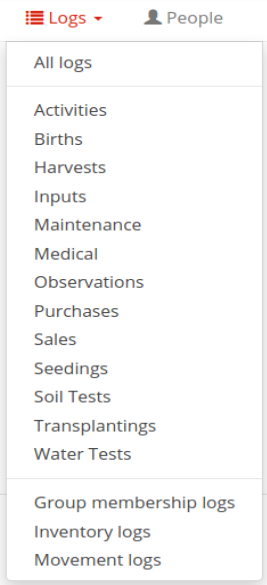
\includegraphics[width=0.3\textwidth]{fig/logs_categories.png}
    \caption{The different categories on logs by default}
    \label{fig:logs_categories}
\end{figure}

We can also find it implements some other features that might come in handy for conveniently recording data. For example, dates autoset by default to the date/time given by the system and each log can be marked ``done/not done''.

\subsubsection{Assets}
Every item that will be recorded in the system, not matter whether it is a log, planted in areas or managed by people. It can also be understood as the ``what''. The default types of assets included in farmOS are compost, planting, animals, equipment and sensors but new types can always be added by adding new modules depending on the requirements.

\subsubsection{Areas}
Areas are not absolutely needed as farmOS can perfectly function without any. However the geographical features it provides will surely be useful for larger farms. It allows to switch between base layers: OpenStreetMap and Google.

\vspace{5mm}
Quite an interesting feature worth mentioning is the \textbf{bed generator}, really useful for further customization as it allows to divide a crop into beds and add more details to each bed.

The bed generator requires two parameters, we need to choose which area is going to be divided into beds and how many beds we want. The width of the beds will be automatically calculated by the generator.

\begin{figure}[H]
    \centering
    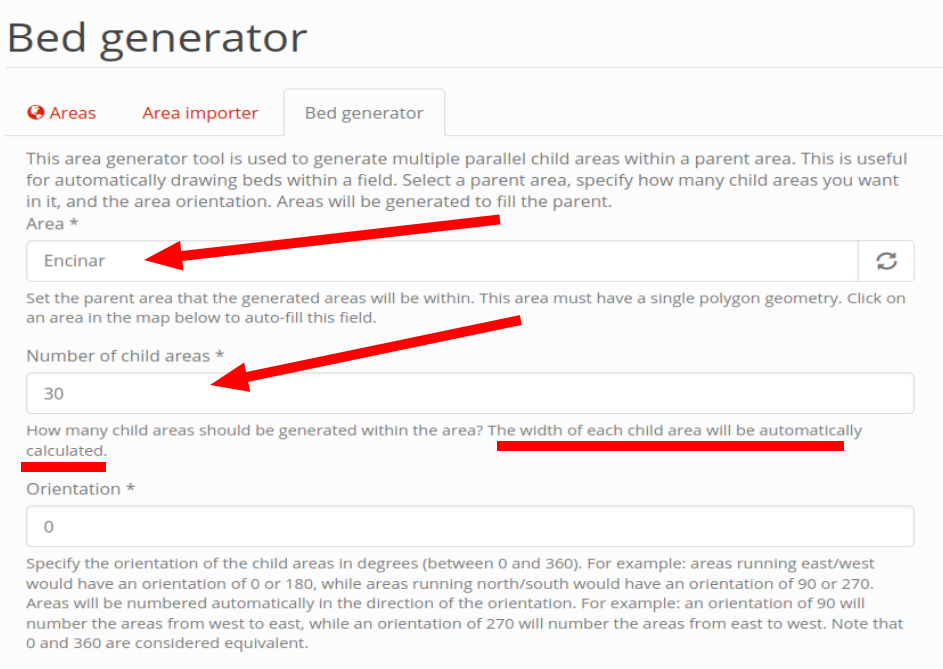
\includegraphics[width=0.9\textwidth]{fig/bed_gen.png}
    \caption{Main view of the bed generator input form}
    \label{fig:bed_gen}
\end{figure}

\begin{figure}[H]
    \centering
    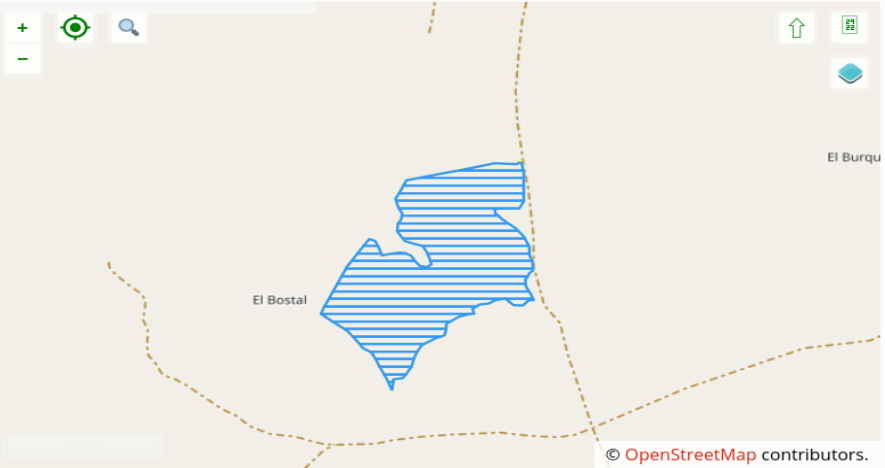
\includegraphics[width=0.85\textwidth]{fig/bed_gen_example.png}
    \caption{An area divided into 30 child areas}
    \label{fig:bed_gen}
\end{figure}

\vspace{5mm}
\subsubsection{People}
Managing people is another useful feature available in farmOS. Three main roles are defined by deafult: manager, worker and viewer,  where the latter has read-only access. The system does not need to be design only around these roles, because of its Drupal modularity, more roles can be defined. However the standarised hosted system does not include more customisation so as not to conflict with a future version.


\begin{figure}[H]
    \centering
    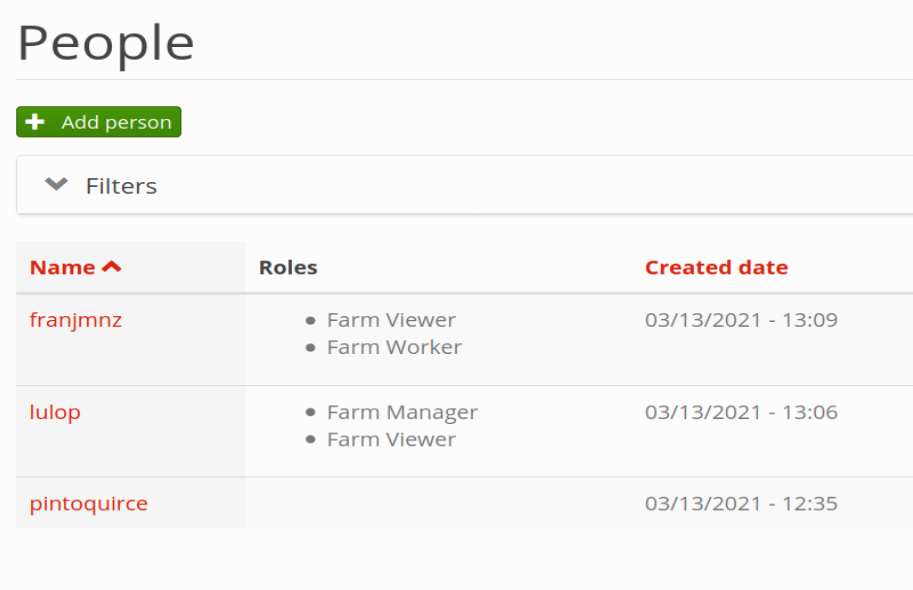
\includegraphics[width=0.8\textwidth]{fig/people.png}
    \caption{Section on different people profiles}
    \label{fig:people}
\end{figure}


\vspace{7mm}
\section{Field kit}
A recent add-on to farmOS main project is the field kit\cite{farmos-fieldkit}. Sometimes, we are in the field and we need to write something down, take a quick note or add an observation. However, going back to the office and launching farmOS to introduce this data seems like a bad decision to make. It is not convenient and it takes way too much time if we find ourselves right in the field.

This is where field kit comes into play. A day to day app that farmers are actually using on the field. This way, farmOS would become a more advanced interface for DB exploration with planning purposes too.

A feature recently implemented for the field kit is the so called ``quick forms'': a simplified set of forms for introducing data into farmOS that allows to create stuff as a shortcut but in the back, will still create a log. Simple annotations can be easily made using these forms. E.g.: eggs harvest


\vspace{7mm}
\section{Sensors}
Let's learn a bit about how sensors\cite{farmos-sensors} work on farmOS, as sensor implementation plays a major role in this thesis.

In order to play with sensors we will have to add the sensor module available, this adds the sensor asset as well as some sub-modules that gives us some more flexibility for integration with external devices.

According to the documentation available online, assembling our own sensors and sending data to farmOS is possible without putting much effort, we would not need to do hard programming or soldering.

The main sub-module implemented by default is Listener. As it is quoted in the sensors section provided by the user guide, ``In addition to manually-entered records, farmOS also provides a framework for receiving data from automated environmental sensors.'' This is mainly what Listener sub-module allows. Although it should not be forgotten that for complex data streams a more customized sub-module may be necessary.

A listener sensor type opens up an endpoint that you post datapost to. Eventually we will basically have an URL associated with the sensor so data can be both requested (in form of a JSON file) from the sensor and authenticated.

\section{Deployment}
By this point, we already know a lot about what is farmOS, how it works, what it is useful for and so on. In the next section we will be deploying farmOS. In this demo we will go through every step of the installation. Then we will start the system and try some of the features.

For simplicity, we will be using a dockerized environment. In the user guide, it is recommended to download the latest release of the pre-packaged farmOS distribution from Drupal.org. We will see all of this in a more detailed way in the next pages.

\section{Conclusions}
At this point, we have adquired a better understanding of the potential that farmOS has. There are infinitely many ways of using a this Drupal distribution, it is really versatile and it can easily be adapted to any project an user may want to develop.

For this project, we will focus on the sensor implementation. We consider that having a sensor set up, while being faily simple, has the potential to save the farmer a significant amount of time as well as collect data that can be crucial for the success of the haverst or the improvement of the ones that are ahead.